\section{Analyse des Marktes}


\subsection{Zielgruppe und potenzielle Kunden}
SemLit richtet sich an alle, die im wissenschaftlichen Bereich tätig sind. Semlit ist eine Dienstleistung, die Wissenschaftler in unterschiedliche Bereichen der Forschung und Entwicklung unterstützen wird. Unsere Kunden können in drei Gruppen gegliedert werden:
\begin{itemize}
\item Private Personen (Studenten und Wissenschaftler)

\item Wissenschaftliche Einrichtungen (Universitäten, Forschungszentren)

\item Unternehmen (Forschungs- und Entwicklungsabteilungen)
\end{itemize}

\subsection{Marktsituation}
Die Marktanalyse wird auf Basis des UNESCO Science Report 2010 durchgeführt. Dieser Bericht stellt wichtige Daten über die Größe, potentielle Entwicklungsrichtungen und Wachstum der Wissenschaft zusammen.\\
Die Endnutzer von SemLit sind Wissenschaftler, weshalb  die potenziellen Entwicklungsrichtungen des Marktes aus den Daten über die Zahl der Wissenschaftler in der Welt abgeleitet werden können. Der Bericht von UNESCO stellt die Daten für die Jahre 2002 und 2007 bereit. Auf dieser Grundlage kann auch das Marktwachstum geschätzt werden.\\

\begin{table}[h!]
  \centering
  \begin{large}
  \begin{tabular}{c}\hline
  \\
  {\color{orange}Die Zahl der Wissenschaftler weltweit}\\
  {\color{orange}hat sich in 5 Jahren }\\
  {\color{orange}von 5.810.700 auf 7.209.700 erhöht.}\\ 
  \\\hline
  \end{tabular}
  \end{large}
\end{table}

Wie man aus Abbildung \ref{fig:fig1} sehen kann, hat sich die gesamte Anzahl der Wissenschaftler in der Welt von 5 810 700 auf 7 209 700 stark erhöht, was einem Wachstum um ca. 24\% in 5 Jahren entspicht. Der größte Anteil sind die Wissenschaftler aus entwickelten Länder, aber Entwicklungsländer zeigen größere Wachstumspotenziale in Höhe von ca. 55,5\% in 5 Jahren, wogegen es in entwickelten Ländern nur etwa  ca. 10,6\% ist.\\
\begin{figure}[h!]
\centering
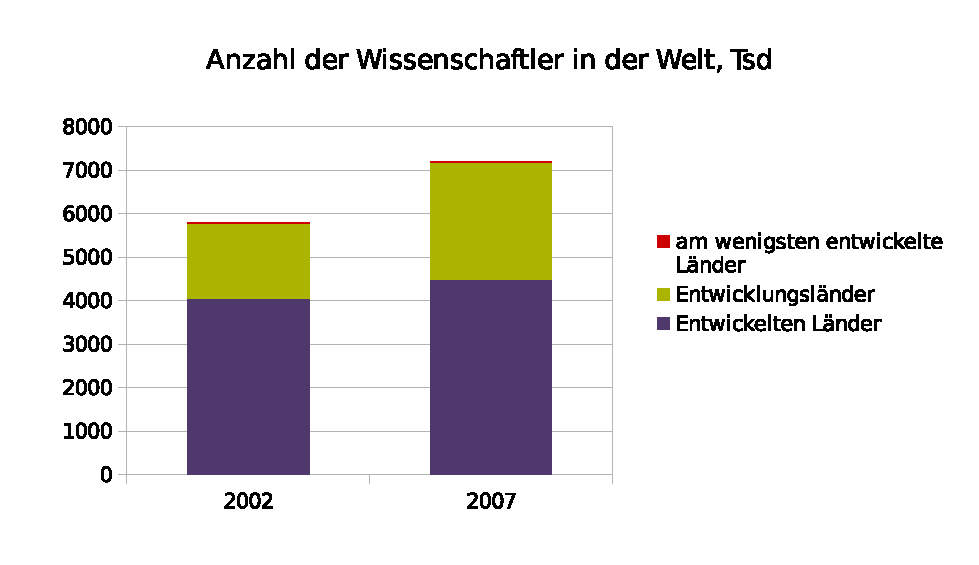
\includegraphics[width=0.8\textwidth]{fig1}
\caption{Zahl der Wissenschaftler weltweit, UNESCO 2010}
\label{fig:fig1}
\end{figure}
Andere Daten, welche die oben genannten Tendenzen bestätigen, beschreiben die Anzahl der Publikationen in der Welt. In 6 Jahre hat sich die Anzahl der Publikationen von 733.305 auf 986.099 erhöht, was ca. 34,5\% Wachstum entspricht. Der größte Anteil entfällt auf die entwickelten Länder, obwohl die Entwicklungsländer ein signifikantes 105,9\% Wachstum zeigen (Abbildung \ref{fig:fig2})\\
\begin{figure}[h!]
\centering
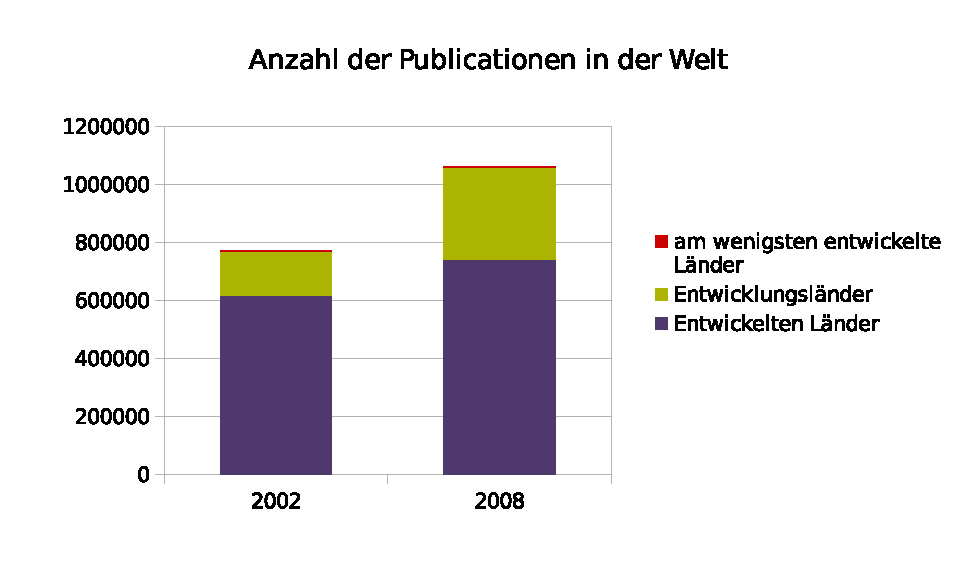
\includegraphics[width=0.8\textwidth]{fig2}
\caption{Anzahl der Publikationen in der Welt, UNESCO 2010}
\label{fig:fig2}
\end{figure}
Auf Grund dieser Daten, kann man feststellen, dass  wichtige Märkte sich in den entwickelten Ländern befinden. Die Entwicklungsländer zeigen jedoch riesige Wachstumspotenziale und werden deshlab nicht außer Acht gelassen. 
Zusammenfassend kann man sagen, dass der Markt potenzieller Kunden in den letzten Jahren ein gutes Wachstum verzeichnet hat und dabei sehr gute Aussichten auf weitere Entwicklung bestehen.

\subsection{Auswahl der regionalen Märkte}
Die Auswahl der regionalen Märkte ist ein wichtiger Teil der Marketingstrategie. Konzentration auf eine begrenzte Liste der regionalen Märkte lässt die regionalen Eigenschaften besser berücksichtigen, um möglichst die besten Dienstleistungen anzubieten. Enge Zusammenarbeit auf dem regionalen Markt und Partnerprogrammene sollten den Erfolg der Absatz unterstützen und neue Richtungen in der Entwicklung darstellen.\\
Um richtige regionale Märkte auszuwählen, werden nur die Länder ausgewählt, die die maximale Anzahl der Wissenschaftler haben, da die Wissenschaftler die Endnutzer von SemLit sind. \\
Die Auswahl der Länder erfolgt mit Hilfe der Angaben von UNESCO 2010 über die Anzahl der Wissenschaftler in jedem Land. Es werden nur die Länder ausgewählt, die zusammen ca. 70\% von der gesamten Anzahl aller Wissenschaftler in der Welt stellen. Die Zusammenfassung der Entwicklung der Anzahl der Wissenschaftler ist in Tabelle \ref{tab:ABC} dargestellt.\\
\begin{table}[h!]
  \centering
  \begin{large}
  \begin{tabular}{c}\hline
  \\
  {\color{orange}Neun ausgewählte Länder stellen}\\
  {\color{orange}ca. 70\% aller SemLit-Kunden weltweit.}\\
  \\\hline
  \end{tabular}
  \end{large}
\end{table}
Wie man aus Tabelle \ref{tab:ABC} sehen kann, machen neun ausgewählte Länder ca. 70\% aller Wissenschaftler in der Welt aus. Viele davon zeigen auch signifikante Wachstumsraten von mehr als 50\% in 5 Jahren. Dazu gehören China und Südkorea.


\begin{table}[h!]
  \centering
  \begin{footnotesize}
  \begin{tabular}{|l|r|r|r|r|r|}\hline
  \textbf{Land} & \multicolumn{4}{ c| }{\textbf{Anzahl der Wissenschaftler, Tsd.}} & \textbf{Wachstum}\\
  & 2002 & \% gesamt & 2007 & \% gesamt & \\ \hline
Welt & 5810.7 & 100.00\% & 7209.7 & 100.00\% & 24.08\% \\ \hline
Vereinigte Staaten & 1342.5 & 23.10\% & 1425.6 & 19.77\% & 6.19\% \\
China & 810.5 & 13.95\% & 1423.4 & 19.74\% & 75.62\% \\
Japan & 646.5 & 11.13\% & 710 & 9.85\% & 9.82\% \\
Russische Föderation & 491.9 & 8.47\% & 469.1 & 6.51\% & -4.64\% \\
Deutschland & 265.8 & 4.57\% & 290.9 & 4.03\% & 9.44\% \\
Vereinigtes Königreich & 198.2 & 3.41\% & 254.6 & 3.53\% & 28.46\% \\
Südkorea & 141.9 & 2.44\% & 221.9 & 3.08\% & 56.38\% \\
Frankreich & 186.4 & 3.21\% & 215.8 & 2.99\% & 15.77\% \\
Kanada & 116 & 2.00\% & 139 & 1.93\% & 19.83 \% \\ \hline
Alle ausgewählten Länder & 4199.7 & 72.28\% & 5150.3 & 71.44\% & 22.63\% \\ \hline
  \end{tabular}
  \end{footnotesize}
  \caption{Länder mit größtem Anteil der Wissenschaftler, basierend auf Daten von UNESCO 2010}
  \label{tab:ABC}
\end{table}


Für alle ausgewählten Länder werden andere wichtige Parameter geschätzt wie z.B. Bruttoinlandsausgaben für Forschung und Entwicklung (GERD) pro Wissenschaftler. Dieser Parameter zeigt, wie viel Geld in die Forschung und Entwicklung investiert wird. Je höher diese Zahl ist, desto höher ist die Wahrscheinlichkeit, dass Wissenschaftler das Geld nicht nur für reine Forschung, sonder auch für Dienstleistungen, die diese Forschung erleichtern könnten, zahlen werden. In Tabelle \ref{tab:ABC2} sind die Angaben zur Entwicklung der Bruttoinlandsausgaben für Forschung und Entwicklung pro Wissenschaftler präsentiert. Wie man aus Tabelle \ref{tab:ABC2} sehen kann, investieren entwickelte Länder sehr viel Geld in Forschung und Entwicklung, was als eine gute Chance für SemLit bewertet werden kann. 
\begin{table}[h!]
  \centering
  \begin{footnotesize}
  \begin{tabular}{|l|p{3cm}|p{3cm}|r|}\hline
  \textbf{Land} & \multicolumn{2}{ r| }{\textbf{GERD pro Wissenschaftler, \$ Tsd.}} & \textbf{Wachstum} \\
  & 2002 & 2007 & \\ \hline
Deutschland & 213.1& 248.4 & 16.56\% \\
Vereinigte Staaten & 206.4 & 243.9 & 18.17\% \\
Japan & 167.3 & 208.4 & 24.57\% \\
Frankreich & 204.7 & 196.1 & -4.20\% \\
Südkorea & 158.6 & 186.3 & 17.47\% \\
Kanada & 165 & 170.7 & 3.45\% \\
Vereinigtes Königreich & 154.6 & 152.2 & -1.55\% \\
China & 48.4 & 72 & 48.76\% \\
Russische Föderation & 32.4 & 50.1 & 54.63\% \\ \hline
  \end{tabular}
  \end{footnotesize}
  \caption{Bruttoinlandsausgaben für Forschung und Entwicklung (GERD) pro Wissenschaftler, basierend auf Daten von UNESCO 2010}
  \label{tab:ABC2}
\end{table} 



\subsection{Schätzung des Marktvolumens}
Schätzung des Marktvolumens ist für den Bereich Wissenschaft nicht einfach, da genauere Daten über die Anzahl und Budget nicht die Realität abbilden können. Deswegen werden diese Daten grob aus vorhandenen Daten abgeleitet. Zuerst wird die gesamt Anzahl der Wissenschaftler und Bruttoinlandsausgaben für Forschung und Entwdie Zahl der Publikationen in Bereich Ingenieurwesen und Technologie, die in diesen Ländern publiziert wurden. 
\begin{table}[h!]
  \centering
  \begin{large}
  \begin{tabular}{c}\hline
  \\
  {\color{orange}Verhältnis Zahl der Wissenschaftler}\\
  {\color{orange}zur Anzahl aller Publikationen ist ca. 7.}\\
  \\\hline
  \end{tabular}
  \end{large}
\end{table}
Aus resultierenden Daten über die Anzahl der Publikationen kann ein Verhältnis-Koeffizient berechnet werden, der eine grobe Schätzung über den Anteil von Ingenieurwesen und Technologie in der gesamten wissenschaftlichen Tätigkeit abgeben kann. Andere Koeffizienten, die wichtig sein könnten, sind Verhältnis von Anzahl der Wissenschaftler/Anzahl aller Publikationen sowie das Verhältnis von Bruttoinlandsausgaben für Forschung und Entwicklung/Anzahl der alle Publikationen. Dieser Koeffizienten zeigen, dass durchschnittlich 7 Wissenschaftler auf eine Publikation arbeiten und durchschnittliche Bruttoinlandsausgaben für eine Publikation ca. 1137,8 Tsd. von PPP\$ ist.
\begin{table}[h!]
  \centering
  \begin{footnotesize}
  \begin{tabular}{|l|l|}\hline
   \textbf{Parameter} &  \textbf{Wert} \\ \hline
  Anzahl der Wissenschaftler & 5150300 \\ \hline
  Bruttoinlandsausgaben für Forschung und Entwicklung & 865,5 Mrd. PPP\$ \\ \hline
  Anzahl der alle Publikationen & 760671 \\ \hline
  Anzahl der Publikationen im Ingenieurwesen & 101351
 \\
  und Technologie& \\ \hline
  Verhältnis (Publikationen in Ing.\& Tech. / alle Publikationen) & 13,3\% \\ \hline
  Verhältnis (Anzahl der Wissenschaftler / Anzahl der & ca. 7 \\
  alle Publikationen ) & \\ \hline
  Verhältnis (Bruttoinlandsausgaben für Forschung & 1137,8 Tsd. PPP\$\\
  und Entwicklung / Anzahl der alle Publikationen) & \\ \hline
  \end{tabular}
  \end{footnotesize}
  \caption{Angaben zu Märkten, basierend auf Daten von UNESCO 2010}
  \label{tab:ABC3}
\end{table}
 

\subsection{Wettbewerber}
Die wesentliche Wettbewerber im Feld der akademischen Suche sind Suchmaschinen. Normalweise bieten Suchmaschinen keine Zugang zum Volltext, sondern nur zum Abstract und den Referenzen. Wichtige Suchmaschine sind in Tabelle \ref{tab:wettSuch} zusammengefasst.
\begin{table}[h!]
  \centering
  \begin{footnotesize}
  \begin{tabular}{|l|l|l|l|}\hline
   \textbf{Name} &  \textbf{Suchverfahren} &  \textbf{Suchbereiche} &   \textbf{Zugang} \\ \hline
BASE - Bielefeld Academic  & Fast Search \& & Interdisziplinär & Kostenfrei \\
Search Engine & Transfer  & & \\ \hline
 Google Scholar & Eigene & Interdisziplinär & Kostenfrei\\\hline
 Microsoft Academic & Vertikale & Informatik & Kostenfrei \\
 Search & Suchmaschine & & \\ \hline
 CiteSeer & Eigene & Informatik & Kostenfrei \\ \hline
  \end{tabular}
    \end{footnotesize}
  \caption{Wichtige Suchmaschine}
  \label{tab:wettSuch}
\end{table} 
 
Zur zweiten Gruppe gehören Datenbanken. Sie stellen nicht nur die Suche in Abstracts und Referenzen bereit, sondern auch Zugang zur Volltexten. Normalweise sind die Suche und der Zugang zum Abstract kostenfrei. Um Zugang zum Volltext zu bekommen, muss das Abonnement zur Datenbank erworben werden. Wichtige Datenbanken sind in der Tabelle \ref{tab:wettDaten} gelistet. 
\begin{table}[h!]
  \centering
    \begin{footnotesize}
  \begin{tabular}{|l|l|l|l|}\hline
  \textbf{Name} &  \textbf{Suchbereiche} &  \textbf{Zugang} &  \textbf{Anbieter} \\ \hline
 SpringerLink & Interdisziplinar & Abonnement & Springer\\ \hline
 Academic Search & Interdisziplinar & Abonnement & EBSCO Publishing\\ \hline
 IEEE Xplore & Informatik \& & Abonnement & IEEE\\ 
 & Elektrotechnik & & \\ \hline
 Scopus & Interdisziplinar & Abonnement & Elsevier\\ \hline
 Web of Science & Interdisziplinar & Abonnement & Thomson ISI \\ \hline
  \end{tabular} 
    \end{footnotesize}
  \caption{Wichtige Datenbanken}
  \label{tab:wettDaten}
\end{table} 


\subsection{Alleinstellungsmerkmal und Kundennutzen}
Der wesentliche Unterschied zwischen SemLit und den bereits existierenden Angeboten auf dem Markt ist die semantische Suche und Verwaltung von Publikationen sowie der Self-Learning Algorithmus, um neue, relevante Publikationen zu finden. Auf der einen Seite stellt SemLit ein Dienstleistung bereit, ähnlich der von Suchmaschinen. Auf der anderen Seite gibt es eine Möglichkeit, auf bevorzugte Datenbanken und Quellen zuzugreifen.\\
SemLit ist sehr flexibel in der Benutzung. Wenn die Kunden bereits existierende Abonnements für eine der Datenbanken haben, kann SemLit als eine erweiterte Suchmaschine genutzt werden. D.h. Kunden können einen glatten Übergang von vorhandener Lösung zu SemLit durchführen oder SemLit als Erweiterung nutzen. 


